\chapter{Transient Performance of Various Geomatric Machines}
\label{C_Kapitel}
\noindent In this chapter we will use the programming language to implement these mathmaticall models from the simple individual machine to multi-machine and attempt to get the transient performance. In the second section, we will try to analysis the difference between this work and another one. 

We choose to use python as the implementation language because python is a interpreted, general-purpose and object-oriented programming language. With its extensive mathmatics library and other third-party library, it is very popular to be used as a scientific scripting language to aid in a numerical data processing and manipulation problem like this.
% #######################################################################

\section{Individual Geomatric Machine}
\noindent Although transient analysis of individual geometric machines with constant parameters has been studied in \cite{meerkov2010transient}, as the basis of all the following models, we still take it as the primary work. Since the performance evaluation method which we try to derive is the foundation of the study in the this paper, we briefly introduce it below.
\begin{figure}[!h]
	\centering
	\includegraphics[]{figures/model_of_one_machine.tikz}
	\caption{State transition diagram of one geometric machine}
	\label{State transition diagram of one geometric machine}
\end{figure}

% simply copy need to reedit

The state transition schema for an individual geometric machine is illustrated in Figure \ref{State transition diagram of one geometric machine}. We use $x_i(n), i \in \{0=down,1=up\}$ to indicate the probability that the machine is in state $i$ during time slot $n$, that is $x_i(n)=Prob[s(n)=i]$. Apparently, the system is described by a two-state ergodic Markov chain and the transformmation of state vector $x(n)=[x_0(n) \quad x_1(n)]^T$ can be described by
\begin{equation}
	x(n+1) = A_1x(n), x_0(n) + x_1(n) =1
\end{equation}
where
\begin{equation} A_1 = \begin{bmatrix} 1-R&P\\R&1-P \end{bmatrix} \end{equation}

% \begin{math}x(n+1)=A_1 x(n)\end{math}
The production rate and consumption rate of an individual machine with the original state both down(0) and up(1) can be calculated as 
\begin{equation} PR(n)=CR(n)=x_1(n)=\begin{bmatrix} 0&1 \end{bmatrix}x(n)=\begin{bmatrix} 0&1 \end{bmatrix}A_1^n
x(0) \end{equation}

the Figure~\ref{Transients of an individual geomatric machine when it is initially down} is the contrast of simulation and calculation of one geometric machine with initial state of down with the parameters of breakdown
probability $P = 0.05$ and repair probability $R = 0.2$.
which are both linear in machine state $x(n)$.

As an illustration, consider a geometric machine with breakdown probability $P=0.05$ and repair probability $R=0.2$. The transients of the system state and the performance measures are given in Figure \ref{Transients of an individual geomatric machine when it is initially down} and \ref{Transients of an individual geomatric machine when it is initially up}, assuming the machine is initially down and up, respectively. As one can see, the initial condition of a machine has strong impact on system transients—which may result in production loss (see Fig. 3) or production gain (see Fig. 4).

\begin{figure*}[!h]
	\centering
	\subfigure[Result of simulation]{
		\includegraphics[width=6.5cm]{figures/individual_s_0.tikz}
		\label{individual simulation down}}
	\subfigure[Result of calculation]{
		\includegraphics[width=6.5cm]{figures/individual_c_0.tikz}	
	 	\label{individual calculation down}}
	\caption{Transients of an individual geomatric machine when it is initially down}
	\label{Transients of an individual geomatric machine when it is initially down}
\end{figure*}

\begin{figure*}[!h]
	\centering
	\subfigure[Result of simulation]{
		\includegraphics[width=6.5cm]{figures/individual_s_1.tikz}
		\label{individual simulation up}}
	\subfigure[Result of calculation]{
		\includegraphics[width=6.5cm]{figures/individual_c_1.tikz}	
	 	\label{individual calculation up}}
	\caption{Transients of an individual geomatric machine when it is initially up}
	\label{Transients of an individual geomatric machine when it is initially up}
\end{figure*}

In the python code, we use the object-oriented features to help build the model. We seperate the codes into two parts. The first part is a class file called Individual. A \pythoninline{class Individual} represents a geomatirc machine that runs in a two-state Markov chain. It holds the parameters, which are transformed from another file, and calculates once a time slot till the end of the time control parameter \pythoninline{n} changes to zero.
\pythonexternal{pycodes/individual/individual.py}
Another file, which is used to call the \pythoninline{class Individual}, are also attached as following. The main purpose of this file is to calculate the the average values of all the evaluation performance in order to get the mathmatical expectation. The final daten are collected in the file called \pythoninline{result.txt}.
\pythonexternal{pycodes/individual/simu1.py}

\section{Transient Performance of Two-Machine Geometric Lines}
\noindent In this Section we also use two part to introduce the two-machine model. It is the most significant difference between two-machine model and individual machine model that there is a buffer between two mahines. This will lead to a performance improvement and other complicated situation.

\subsection{Mathematical Dirivation of two-machine Model}
\label{mathematical two machine}
\noindent Suppose that we have a two-machine geometric line restrained by assumptions 1-8. shown in Figure \ref{State transition diagram of two geometric machine with buffer}. From the figure we can easily tell that the system obersve an ergodic Markov chain. Moreover, to machine state $s_i(n)$, we use $j(n)$ to imply the number of products in the buffer at the start of time slot $n$. Then, the state of the Markov chain can be described by a triple $(j(n),s_1(n),s_2(n))$, where $j(n)\in {0,1,...,N}$ and $s_1(n),s_2(n) \in {0,1}$. Apparently, the system will in total have states of $4(N+1)$.In order derive the transition probabilities from these states, we organize the states in the following form: we use $r(j,s1,s2)$ indicate the state number of the Markov chain state $(j,s_1,s_2)$, $h\in {0,1,...,N}, s_1,s_2\in {0,1}$. Given
\begin{equation}
	r(j,s_1,s_2) = 4j + 2s_1 +s_2 +1 .
	\label{definition of r}
\end{equation}
\begin{figure}[!h]
	\centering
	\includegraphics[]{figures/model_of_two_machine_with_buffer.tikz}
	\caption{State transition diagram of two geometric machine with buffer}
	\label{State transition diagram of two geometric machine with buffer}
\end{figure}
Then, the sequence of the $4(N+1)$ system states can be described in Table \ref{two machine state}. Moreover, we use a unique number from $1$ to $4(N+1)$ to represent each system state. For instance, State $1$ represents that both machines are broken down and the buffer is empty, while State $4(N+1)$ represents that both machines are working properly and the buffer is full. Furthermore, suppose a state number $r$, its related buffer and machines states can be described as follows:
\begin{equation}
	\begin{aligned}
		j^{(r)} =& \lf{\frac{r-1}{4}}\rf, s_1^{(r)} = \lf{\frac{r-1-4j^{(r)}}{2}}\rf \\
		s_2^{(r)} =& \lf{\frac{r-1-4j^{(r)-2s_1^{(r)}}}{1}}\rf
	\end{aligned}
\end{equation}
where $\lf{a}\rf$ refers to the largest integer not greater than $a$.
\begin{table}[H]
	\centering
	\caption{Arrangement of the System States $k = 0,1,...,N$}
	\begin{tabular}{c|llll}\hline
		State number$(r)$&$4k+1$ & $4k+2$  & $4k+3$ &  $4k+4$   \\\hline
		$j$   & $k$          & $k$      & $k$   &  $k$   \\
		$s_1$ & $0$          & $0$      & $1$   &  $1$ \\
		$s_2$ & $0$          & $1$      & $0$   &  $1$  \\ \hline
	\end{tabular}
	\label{two machine state}
\end{table}
Notice that the transition of $j(n)$ is deterministic defined by $s_1(n)$ and $s_2(n)$. For a given serial production lines, the equations that characterize the dynamics of $j(n)$ have been formulated in \cite{zhang2013transient}
\begin{equation}
	j(n+1)=j'(n) + s_1(n)min\{N-j'(n),1\}
	\label{number in buffer}
\end{equation}
where
\begin{equation}
	j'(n)=j(n)-s_2(n)min\{j(n),1\}
\label{occupation of buffer}
\end{equation}
In the above equtions, $j'(n)$ refers to the occupancy of the buffer as long as machine $m_2$ takes a part from the buffer at the start of time slot $n$.

The transitions of $s_i(n)$'s, meanwhile, are probabilistic based on \ref{transition probabilities}. Thus, we can view each of the $4(N+1)$ states, then, coming from \ref{number in buffer} and \ref{occupation of buffer}, distinguish all possible aimed states after one time slot by enumerating all four combining ways of $s_1(n)$ and $s_2(n)$, and, in the end, measure the corresponding transition probabilities using \ref{transition probabilities}. Suppose that we use $A_2$ to characterize the transition probability matrix derived and use $x_i(n)$, $i\in {1,2,...,4(N+1)}$, describe the probability that the system, in other words, the Markov chain, is in state $i$ in the period of the time slot $n$. Furthermore, the evolution of the system state, $x(n)=[x_1(n)x_2(n)...x_4(N+1)^{(n)}]^T$, is derived by
\begin{equation}
	x(n+1) = A_2x(n), \sum_{i=1}^{4(N+1)} x_i(n) = 1 .
\end{equation}
According the state arrangement \ref{definition of r}, we have
\begin{equation}
	\begin{aligned}
		x_{4j+1}(n)=&\text{Prob[$m_1$ down, $m_2$ down, buffer $b$ has $j$ parts at time $n$]}  \\
		x_{4j+2}(n)=&\text{Prob[$m_1$ down, $m_2$ up, buffer $b$ has $j$ parts at time $n$]}  \\
		x_{4j+3}(n)=&\text{Prob[$m_1$ up, $m_2$ down, buffer $b$ has $j$ parts at time $n$]} \\
		x_{4j+4}(n)=&\text{Prob[$m_1$ up, $m_2$ up, buffer $b$ has $j$ parts at time $n$]}.
	\end{aligned}
\end{equation}
Thus, according to the definitions derived in \ref{performance measures}, we can compute the performance measures of the two-machine geometric line system in the following way:
\begin{equation}
	\begin{aligned}
		PR(n)=&\  \text{Prob[$m_2$ up,buffer $b$ not empty during time $n$] }\\
		=&\ C_1x(n)=[C_{1,0}\ C_{1,1}\ ...\ C_{1,N}]x(n) \\
		CR(n)=&\ \text{Prob[m1 up and not blocked during time n]} \\
		=&\ C_2x(n)=[C_{2,0}\ C_{2,1}\ ...\ C_{2,N}]x(n)\\
		WIP(n)=&\ \sum_{i=1}^N i \cdot \text{Prob[buffer $b$ has $i$ parts at time $n$]} \\
		=&\ C_3x(n)=[C_{3,0}\ C_{3,1}\ ...\ C_{3,N}]x(n) \\
		ST_2=&\ \text{Prob[$m_2$ up and buffer $b$ empty at time $n$]} \\
		=&\ C_4x(n)=[C_{4,0}\ C_{4,1}\ ...\ C_{4,N}]x(n) \\
		BL_1=&\ \text{Prob[$m_1$ up, $m_2$ down,buffer $b$ is full at time $n$]} \\
		=&\  C_5x(n)=[C_{5,0}\ C_{5,1}\ ...\ C_{5,N}]x(n)
	\end{aligned}
\end{equation}
where
\begin{equation}
    \begin{aligned}
        C_{1,0}\ &= \ [0 0 0 0],  &C_{1,i}&= [0 1 0 1],  &i&= 1,...,N \\
        C_{2,N}\ &=\ [0 0 0 1],  &C_{2,i}&= [0 0 1 1],  &i&= 0,..,N-1 \\
        C_{3,i}\ &=\ [i i i i],  &i&=  0,...,N \\
        C_{4,0}\ &=\ [0 1 0 1],  &C_{4,i}&= [0 0 0 0],  &i&= 1,...,N  \\
        C_{5,N}\ &=\ [0 0 1 0],  &C_{5,i}&= [0 0 0 0],  &i&= 0,...,N-1
    \end{aligned}
\end{equation}
In consequence, all these performance measures can be described as linear related in system state $x(n)$.

As an example, suppose a two-machine geometric line given by ssumptions 1-8. with machine and buffer parameters
\begin{displaymath}
	P_1=0.03, R_1=0.18, P_2=0.06, R_2=0.21, N=10.
\end{displaymath}
Presume that both machines are initially broken and the buffer in the middle is initially empty. The Figure \ref{Transients of a two-machine geometric line} presents transients of the performance measures of this system. For both machines are initially down and the buffer is empty, $PR(n)$,$ CR(n)$ and $WIP(n)$ all rise from $0$. Moreover, $PR(n)$ and $CR(n)$ have significant difference during the transient process, while with $n$ growing larger, both converge to the same value because of the conservation of flow in steady state. In addition, for the buffer is empty in the beginning, $BL_1(n)$ stays zero (in other words, machine $m_1$ is not in blockage state) until $n > N$.

\begin{figure*}[!h]
	\centering
	\subfigure[]{
		\includegraphics[width=0.45\linewidth,height=0.35\linewidth]{figures/two_machine_pr_and_cr.tikz}
		\label{two machine pr and cr}}
	\subfigure[]{
		\includegraphics[width=0.45\linewidth,height=0.35\linewidth]{figures/two_machine_wip.tikz}	
		 \label{two machine wip}}
	\subfigure[]{
		\includegraphics[width=0.45\linewidth,height=0.35\linewidth]{figures/two_machine_bl_and_st.tikz}	
		\label{two machine bl and st}}
	\caption{Transients of a two-machine geometric line. (a) $PR(n)\ and\ CR(n)$;(b) $WIP(n)$; (c) $ST_2(n)\ and\ BL_2(n)$}
	\label{Transients of a two-machine geometric line}
\end{figure*}


\subsection{Implementation of two-machine model}
\label{c}
\noindent In the python platform, we still keep the \pythoninline{class Individual} and have a slight adjust to simulate a machine instance. The main modification is to add two instance to represent the buffer upstream and downstream respectively. Moreover, it also hold a flag to judge whether the machine is blocked or starved according to the state of buffer in up- and downstream so that it cannot process a part in a time slot. Meanwhile, we add another \pythoninline{class Buffer} to represent the buffer in the middle of two machines. The buffer have its own storage to denote the numbers of products it hold and the maximal capacity. In addition, it also implements the products receiving and taking away function by two method \pythoninline{add_one() } and \pythoninline{take_one()}.

We use an UML diagram (Figure \ref{two machine uml}) to describe the relationship between three class. The program procedure is as follow: first, in the script ''sim2.py'' create we a certain amount of production lines, and each contains an instance from \pythoninline{class TwoMachine}. Meanwhile, the \pythoninline{class TwoMachine} consists of two instances from \pythoninline{class Individual} which represent the first and second machine respectively, and a buffer instance from \pythoninline{class Buffer}. In addition, the function \pythoninline{one_slot()} simulate a process in one time slot, and then give the critical transient performance measures back  to script ''sim2.py'' in order that the data can be record in the file.

\begin{figure*}[!h]
	\centering
	\includegraphics[width=0.8\linewidth]{two_machine.png}
	\caption{UML diagram of a two-machine model}
	\label{two machine uml}
\end{figure*}
\section{Transient Performance of Multi Machine Lines}
\noindent In this section we extend the two-machine model to multi-machine model. The model now can be used with arbitrary numbers of machines and buffers composition. The importanet problem that we need to solve, is to arrange the operations that in one time slot the machines and buffers should do.

\subsection{Mathematical Dirivation of multi-machine Model}
\noindent Suppose we have an $M$-machine geometric line observing assumptions 1-8. Because the geometric distribution obey the memoryless attribute, the system can still be described by a Markov chain. Use $j_i(n)$ to indicate the number of parts in buffer $b_i$ at the start of time slot $n$. Moreover, we can describe the state of Markov chain with vector $(j_1(n), ... , j_{M-1}(n)$, $ s_1(n), ..., s_M(n))$, where $j_i(n) \in {0, 1, ...,N_i}, i = 1, ..., M-1$, and $s_i(n) \in {0, 1}, i = 1, ..., M$. Apparently, the system has totally states of $S = 2^M \sum^{M-1}_{i=1} (N_i + 1)$. To derive the transition probabilities among these states, the same approach described in Section \ref{mathematical two machine} is applied to linearize the state space. Particularly, the states from State 1 to S are arranged in the following manner: $r(j_1, ..., j_{M-1}, s_1, ..., s_M)$ refer to the state number of the Markov chain state $(j_1, ..., j_{M-1}, s_1, ..., s_M)$. Define
\begin{equation}
    r(j_1,...,j_{M-1},s_1,...,s_m) = 1+\sum^{M-1}_{i=1}j_i\alpha _i + \sum^M_{i=1}s_i\beta _i
    \label{multimachine r}
\end{equation}
where
\begin{align*}
    \alpha_i &= \left\{ 
      \begin{aligned} &2^M \ \prod^{M-1}_{h=i+1}(N_h + 1),  &i &= 1,...,M-2 \\ &2^M \ , &i &= M-1 
      \end{aligned}
    \right. 
    \\ \beta _i &= 2^{M-1}, i = 1,...,M
  \end{align*}
  In this regulation, each state can be arranged a individual number between 1 and S. On the contrary, consider the state number $r$ of a system state, $r\in{1, .., S}$, the corresponding machine state $s^{(r)}_i ,  i = 1, ..., M$, and buffer state, $j^{(r)}_i , i = 1,..., M-1$, can be derived as follows:

\begin{equation}
    j^{(r)}_i = \left\{
\begin{aligned}
    &\lf{\frac{r-1}{\alpha_1}}\rf, &i&=1 \\ &\lf{\frac{r-1-\sum^{i-1}_{h-1}j^{(r)}_h\alpha_h}{\alpha_i}}\rf, &i&=2,...,M-1
\end{aligned}    
\right.
\end{equation}

\begin{equation}
    s_i^{(r)}=\left\{
    \begin{aligned}
        &\lf{\frac{r-1-\sum^{M-1}_{h-1}j^{(r)}_h\alpha_h}{\beta_1}}\rf, &i&=1 \\ &\lf{\frac{r-1-\sum^{M-1}_{h-1}j^{(r)}_h\alpha_h-\sum^{i-1}_{h-1}s^{(r)}_h\beta_h}{\beta_i}}\rf, &i&=2,...,M
    \end{aligned}\right.
\end{equation}

As is shown above, compared to the two-machine production lines model, the state arrangement of both system are very similar, but in this term with enlarged state it can accomodate more buffers and machines.

Alike with the two-machine situation, the transitions of $j_i(n)$'s are deterministic with machine state $s_1(n),...,s_M(n)$, and can be computed according to the following equations:
\begin{equation}
    \begin{aligned}
      j_i(n + 1) &= j'_i(n) + s_i(n)min\{j_{i-1}(n),N_i - j'_i(n), 1\} \\
      i &= 2, ..., M - 1 \\
      j_1(n + 1) &= j'_1(n) + s_1(n)min\{N_1 - j'_1(n), 1\}
    \end{aligned}
    \end{equation}
    where
    \begin{equation}
      \begin{aligned}
      j'_{M-1}(n)&=j_{M-1}(n) - s_M(n)min\{j_{M-1}(n), 1\} \\
    j'_i(n)&=j_i(n)- s_{i+1}(n)min\{j_i(n),N{i+1}-j'{i+1}(n), 1\} \\
     i &= 1, . . . , M - 2.
    \end{aligned}
    \end{equation}
In the above equtions, $j'_i(n)$ indicates the occupancy of buffer $b_i$ as loog as machine $m_{i+1}$ takes a products  from $b_i$ at the start of time slot $n$.

Subsequently, according to the state number derived in \ref{multimachine r} all $S$ system states from $1$ to $S$ and describe $x_i(n) = $ Prob[System in state $i$ in time slot $n$]. Afterwards, the procedure of the state transformation of the Markov chain, $x(n) = [x_1(n)x_2(n)...x_S(n)]^T$, can be derived by
\begin{equation}
    x(n+1) = A_Mx(n), \sum^S_{i=1}x_i(n) = 1.
\end{equation}

The transient perfomrmace of the system can be given by

\begin{equation}
    \begin{aligned}
  PR(n) &= \text{Prob}[m_M \text{up and} b_{M-1} \text{not empty at time slot} n] \\
        &= \text{Prob}[s_M(n) = 1 \text{and} j_{M-1}(n) > 0] \\
        &=D_1x(n) = [d_{1,1}d_{1,2}...d_{1,S}]x(n) \\
  CR(n) &= \text{Prob}[m_1 \text{is up and not blocked at time slot} n] \\
        &= D_2x(n) = [d_{2,1}d_{2,2}...d_{2.S}]x(n) \\
WIP_i(n) &=\sum^{N_i}_{k=1}k\cdot \text{Prob}[j_i(n)=k] \\
        &= D_{3,i}x(n) = [d_{3,1}d_{3,2}...d_{3.S}]x(n), i=1,...,M-1 \\
ST_i(n) &=  \text{Prob}[m_i \text{up and} b_{i-1} \text{empty at time slot} n] \\
        &= \text{Prob}[s_i(n) = 1 \text{and} j_{i-1}(n) = 0] \\
        &= D_{4,i}x(n) = [d_{4,1}d_{4,2}...d_{4.S}]x(n), i=2,...,M \\
BL_i(n) &=  \text{Prob}[m_i \text{up} b_{i} \text{full, and} m_{i+1}\text{down or blocked at time slot} n] \\
        &= D_{5,i}x(n) = [d_{5,1}d_{5,2}...d_{5.S}]x(n), i=1,...,M-1
     \end{aligned}
\end{equation}
where
\begin{align*}
    d_{1,r} &= \left\{\begin{aligned}  &1, \text{if}s^{(r)}_M = 1 \text{and} j^{(r)}_{M-1}  > 0 \\ &0, otherwise
    \end{aligned}\right. \\
    d_{2,r} &= 1- d_{5,1,r} \\
    d_{3,i,r} &= j^{(r)}_i, i = 1,...,M-1,  r = 1,...,S \\
    d_{4,i,r} &= \left\{\begin{aligned} &1, \text{if} s^{(r)}_i = 1 \text{and} j^{(r)}_{i-1}=0 \\ &0 , otherwise
    \end{aligned}\right. \\
    d_{5,i,r} &= \left\{\begin{aligned} & d_{5,i+1,r},  &\text(if) s^{(r)}_i &=1,s^{(r)}_{i+1} =1, \text{and} j^{(r)}_i = N_i \\  & 1,  &\text(if) s^{(r)}_i &=1,s^{(r)}_{i+1} =0, \text{and} j^{(r)}_i = N_i \\ & 0, &otherwise
    \end{aligned}\right.
  \end{align*}
  in other words, $d_{1,r},d_{2,r}, d_{3,i,r}, d_{4,i,r}$ and $d_{5,i,r}$ represent the $r$th element in vectors $D_1,D_2,$ $D_{3,i},D_{4,i}$ and $D_{5,i}$, separately. Apparently, in system state $x(n)$ all the performance measures are linear.

  As an instance, suppose a four-machine geometric line obeying the assumptions 1-8. with machines and buffer parameters
  \begin{displaymath}
      P_i = 0.05, R_i-0.2, i = 1,...4; N_i = 5, i=1,...3.
  \end{displaymath}

  Presume that all machines are broken down in the beginning and buffers are all empty either. The transient performance of this system are shown in Figure \ref{Transients of a four-machine geometric line}.


\begin{figure*}[!h]
	\centering
	\subfigure[]{
		\includegraphics[width=0.45\linewidth,height=0.35\linewidth]{figures/four_machine_pr_and_cr.tikz}
		\label{four machine pr and cr}}
	\subfigure[]{
		\includegraphics[width=0.45\linewidth,height=0.35\linewidth]{figures/four_machine_wip.tikz}	
		 \label{four machine wip}}
	\subfigure[]{
		\includegraphics[width=0.45\linewidth,height=0.35\linewidth]{figures/four_machine_st.tikz}	
		\label{four machine st}}
	\subfigure[]{
		\includegraphics[width=0.45\linewidth,height=0.35\linewidth]{figures/four_machine_bl.tikz}	
		\label{four machine bl}}
	\caption{Transients of a four-machine geometric line. (a) $PR(n) \ and\ CR(n)$;(b) $WIP(n)$; (c) $ST_i(n)$;(d) $BL_i(n)$.}
	\label{Transients of a four-machine geometric line}
\end{figure*}

\subsection{Implementation of multi-machine model}
\noindent In the python platform, it is also very similar to two-machine model in section \ref{Transients of a four-machine geometric line}. The \pythoninline{class Individual} and \pythoninline{class Buffer} are also keeped to represent one machine instance and one buffer instance, while they are reorganized in new \pythoninline{class MultiMachine}. In addition, in each \pythoninline{MultiMachine} instance it contains two arrays named as \pythoninline{Machine} and \pythoninline{BufferArray} respectively. The formor array contains a number of \pythoninline{MachineNumber} machines while the latter array holds one less buffer compared to the formor array. 

We use a UML diagram to illustrate the relationship between these class, see Figure \ref{multi machine uml}. In script ''sim4.py'' we initialize all the given parameters and create enough instances of \pythoninline{class MultiMachine}. Therefore, in each time slot the critical transient performance measures are collected from function \pythoninline{one_slot()}, and in the end write in the file.

\begin{figure*}[!h]
	\centering
	\includegraphics[width=0.8\linewidth]{multi_machine.png}
	\caption{UML diagram of a multi-machine model}
	\label{multi machine uml}
\end{figure*}

\section{Result Analysis}
\noindent There's no apparently difference between the work of this paper and \cite{chen2015transient} in one machine mode, but it shows difference in two-machine lines especially in $ST_2(n)$ and $BL_1$ these two parameters. From the Figure \ref{2_c} can we tell the differece. And in the four-machine lines model there are more difference shown in Figure \ref{differece four}.


% a significant difference can be found between the Figure~\ref{two machine bl and st} and the original Figure~\ref{st_bl_origin}


\begin{figure*}[!h]
	\centering
	\includegraphics[width=0.5\linewidth]{2_c.png}
	\caption{Performance contrast of a two-machine geometric line $ST_2(n) \ and\ BL_2(n)$}
	\label{2_c}
\end{figure*}

\begin{figure*}[!h]
	\centering
	\subfigure[]{
		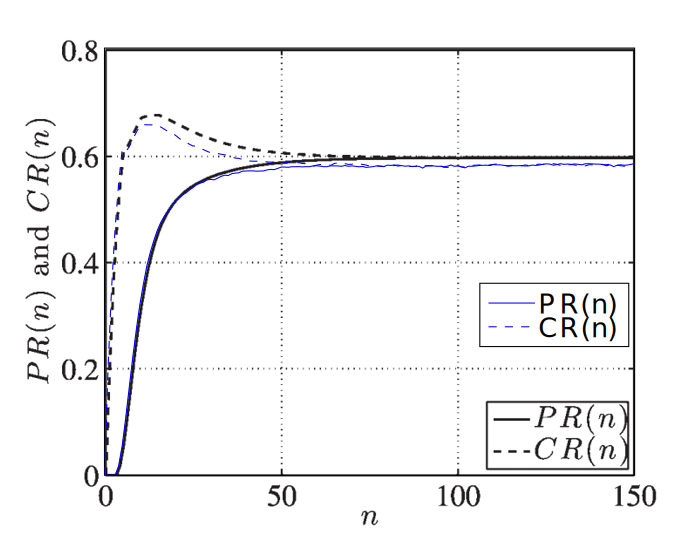
\includegraphics[width=0.45\linewidth,height=0.35\linewidth]{4_a.png}
		\label{d four machine pr and cr}}
	\subfigure[]{
		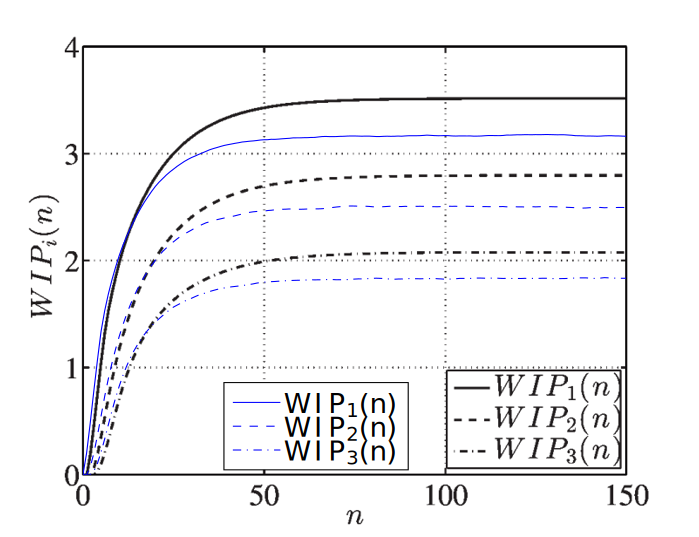
\includegraphics[width=0.45\linewidth,height=0.35\linewidth]{4_b.png}	
		 \label{d four machine wip}}
	\subfigure[]{
		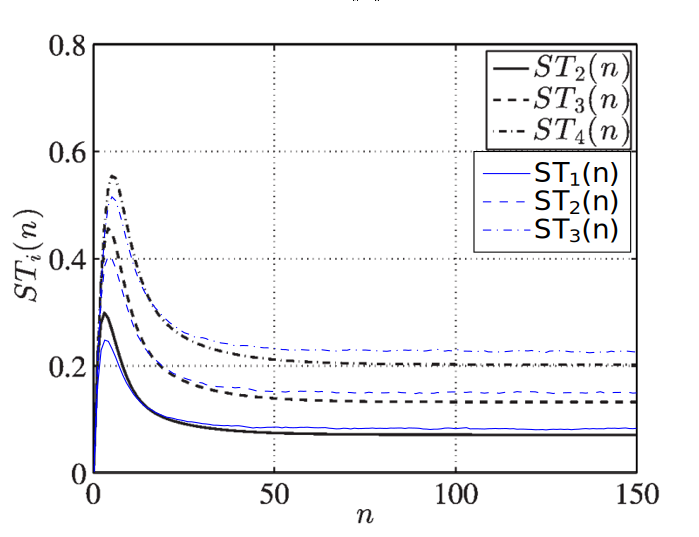
\includegraphics[width=0.45\linewidth,height=0.35\linewidth]{4_c.png}	
		\label{d four machine st}}
	\subfigure[]{
		\includegraphics[width=0.45\linewidth,height=0.35\linewidth]{4_d.png}	
		\label{d four machine bl}}
	\caption{Transients of a four-machine geometric line. (a) $PR(n) \ and\ CR(n)$;(b) $WIP(n)$; (c) $ST_i(n)$;(d) $BL_i(n)$.}
	\label{differece four}
\end{figure*}

For the reasons of these difference, we suppose a few points: First, we doubt that whether the lack of enough quantity of samples cause the problem. But when we enlarege the quantity of simulation time from 10000 to 100000, we found no apparent difference from the result. Second, due to that we don't know what kind of programming language the reseachers coding with, a probable cause may be we take a different platform to programm with, and that may cause some accuracy problem. Third, we also doubt that the researchers may do some kind of curve smoothing in oder to present a perfect result.